% Options for packages loaded elsewhere
\PassOptionsToPackage{unicode}{hyperref}
\PassOptionsToPackage{hyphens}{url}
%
\documentclass[
]{article}
\usepackage{amsmath,amssymb}
\usepackage{iftex}
\ifPDFTeX
  \usepackage[T1]{fontenc}
  \usepackage[utf8]{inputenc}
  \usepackage{textcomp} % provide euro and other symbols
\else % if luatex or xetex
  \usepackage{unicode-math} % this also loads fontspec
  \defaultfontfeatures{Scale=MatchLowercase}
  \defaultfontfeatures[\rmfamily]{Ligatures=TeX,Scale=1}
\fi
\usepackage{lmodern}
\ifPDFTeX\else
  % xetex/luatex font selection
\fi
% Use upquote if available, for straight quotes in verbatim environments
\IfFileExists{upquote.sty}{\usepackage{upquote}}{}
\IfFileExists{microtype.sty}{% use microtype if available
  \usepackage[]{microtype}
  \UseMicrotypeSet[protrusion]{basicmath} % disable protrusion for tt fonts
}{}
\makeatletter
\@ifundefined{KOMAClassName}{% if non-KOMA class
  \IfFileExists{parskip.sty}{%
    \usepackage{parskip}
  }{% else
    \setlength{\parindent}{0pt}
    \setlength{\parskip}{6pt plus 2pt minus 1pt}}
}{% if KOMA class
  \KOMAoptions{parskip=half}}
\makeatother
\usepackage{xcolor}
\usepackage[margin=1in]{geometry}
\usepackage{color}
\usepackage{fancyvrb}
\newcommand{\VerbBar}{|}
\newcommand{\VERB}{\Verb[commandchars=\\\{\}]}
\DefineVerbatimEnvironment{Highlighting}{Verbatim}{commandchars=\\\{\}}
% Add ',fontsize=\small' for more characters per line
\usepackage{framed}
\definecolor{shadecolor}{RGB}{248,248,248}
\newenvironment{Shaded}{\begin{snugshade}}{\end{snugshade}}
\newcommand{\AlertTok}[1]{\textcolor[rgb]{0.94,0.16,0.16}{#1}}
\newcommand{\AnnotationTok}[1]{\textcolor[rgb]{0.56,0.35,0.01}{\textbf{\textit{#1}}}}
\newcommand{\AttributeTok}[1]{\textcolor[rgb]{0.13,0.29,0.53}{#1}}
\newcommand{\BaseNTok}[1]{\textcolor[rgb]{0.00,0.00,0.81}{#1}}
\newcommand{\BuiltInTok}[1]{#1}
\newcommand{\CharTok}[1]{\textcolor[rgb]{0.31,0.60,0.02}{#1}}
\newcommand{\CommentTok}[1]{\textcolor[rgb]{0.56,0.35,0.01}{\textit{#1}}}
\newcommand{\CommentVarTok}[1]{\textcolor[rgb]{0.56,0.35,0.01}{\textbf{\textit{#1}}}}
\newcommand{\ConstantTok}[1]{\textcolor[rgb]{0.56,0.35,0.01}{#1}}
\newcommand{\ControlFlowTok}[1]{\textcolor[rgb]{0.13,0.29,0.53}{\textbf{#1}}}
\newcommand{\DataTypeTok}[1]{\textcolor[rgb]{0.13,0.29,0.53}{#1}}
\newcommand{\DecValTok}[1]{\textcolor[rgb]{0.00,0.00,0.81}{#1}}
\newcommand{\DocumentationTok}[1]{\textcolor[rgb]{0.56,0.35,0.01}{\textbf{\textit{#1}}}}
\newcommand{\ErrorTok}[1]{\textcolor[rgb]{0.64,0.00,0.00}{\textbf{#1}}}
\newcommand{\ExtensionTok}[1]{#1}
\newcommand{\FloatTok}[1]{\textcolor[rgb]{0.00,0.00,0.81}{#1}}
\newcommand{\FunctionTok}[1]{\textcolor[rgb]{0.13,0.29,0.53}{\textbf{#1}}}
\newcommand{\ImportTok}[1]{#1}
\newcommand{\InformationTok}[1]{\textcolor[rgb]{0.56,0.35,0.01}{\textbf{\textit{#1}}}}
\newcommand{\KeywordTok}[1]{\textcolor[rgb]{0.13,0.29,0.53}{\textbf{#1}}}
\newcommand{\NormalTok}[1]{#1}
\newcommand{\OperatorTok}[1]{\textcolor[rgb]{0.81,0.36,0.00}{\textbf{#1}}}
\newcommand{\OtherTok}[1]{\textcolor[rgb]{0.56,0.35,0.01}{#1}}
\newcommand{\PreprocessorTok}[1]{\textcolor[rgb]{0.56,0.35,0.01}{\textit{#1}}}
\newcommand{\RegionMarkerTok}[1]{#1}
\newcommand{\SpecialCharTok}[1]{\textcolor[rgb]{0.81,0.36,0.00}{\textbf{#1}}}
\newcommand{\SpecialStringTok}[1]{\textcolor[rgb]{0.31,0.60,0.02}{#1}}
\newcommand{\StringTok}[1]{\textcolor[rgb]{0.31,0.60,0.02}{#1}}
\newcommand{\VariableTok}[1]{\textcolor[rgb]{0.00,0.00,0.00}{#1}}
\newcommand{\VerbatimStringTok}[1]{\textcolor[rgb]{0.31,0.60,0.02}{#1}}
\newcommand{\WarningTok}[1]{\textcolor[rgb]{0.56,0.35,0.01}{\textbf{\textit{#1}}}}
\usepackage{longtable,booktabs,array}
\usepackage{calc} % for calculating minipage widths
% Correct order of tables after \paragraph or \subparagraph
\usepackage{etoolbox}
\makeatletter
\patchcmd\longtable{\par}{\if@noskipsec\mbox{}\fi\par}{}{}
\makeatother
% Allow footnotes in longtable head/foot
\IfFileExists{footnotehyper.sty}{\usepackage{footnotehyper}}{\usepackage{footnote}}
\makesavenoteenv{longtable}
\usepackage{graphicx}
\makeatletter
\def\maxwidth{\ifdim\Gin@nat@width>\linewidth\linewidth\else\Gin@nat@width\fi}
\def\maxheight{\ifdim\Gin@nat@height>\textheight\textheight\else\Gin@nat@height\fi}
\makeatother
% Scale images if necessary, so that they will not overflow the page
% margins by default, and it is still possible to overwrite the defaults
% using explicit options in \includegraphics[width, height, ...]{}
\setkeys{Gin}{width=\maxwidth,height=\maxheight,keepaspectratio}
% Set default figure placement to htbp
\makeatletter
\def\fps@figure{htbp}
\makeatother
\setlength{\emergencystretch}{3em} % prevent overfull lines
\providecommand{\tightlist}{%
  \setlength{\itemsep}{0pt}\setlength{\parskip}{0pt}}
\setcounter{secnumdepth}{5}
\usepackage{ctex}

%\usepackage{xltxtra} % XeLaTeX的一些额外符号
% 设置中文字体
%\setCJKmainfont[BoldFont={黑体},ItalicFont={楷体}]{新宋体}

% 设置边距
\usepackage{geometry}
\geometry{%
  left=2.0cm, right=2.0cm, top=3.5cm, bottom=2.5cm} 

\usepackage{amsthm,mathrsfs}
\usepackage{booktabs}
\usepackage{longtable}
\makeatletter
\def\thm@space@setup{%
  \thm@preskip=8pt plus 2pt minus 4pt
  \thm@postskip=\thm@preskip
}
\makeatother
\ifLuaTeX
  \usepackage{selnolig}  % disable illegal ligatures
\fi
\usepackage[]{biblatex}
\usepackage{bookmark}
\IfFileExists{xurl.sty}{\usepackage{xurl}}{} % add URL line breaks if available
\urlstyle{same}
\hypersetup{
  hidelinks,
  pdfcreator={LaTeX via pandoc}}

\author{}
\date{\vspace{-2.5em}}

\begin{document}

{
\setcounter{tocdepth}{2}
\tableofcontents
}
\section{R语言教程!compareGroups神包制作描述性表一}\label{compare}

\begin{quote}
第95期 R语言教程!compareGroups神包制作描述性表一

描述性表1在论文写作中占据着开篇起笔的作用。\textbf{对所用的数据进行描述和简单分析,为后续的模型构建提供数据可靠性信息}

本期介绍如何使用compareGroups神包来快速生成符合学术规范的表1。并进行包括以下自定义设置:1\textbf{.设置亚组 2.设置非正态变量使用非参组间检验 3.设置显示缺失值 4.设置显示OR值 5.设置使用自定义组间比较方法 6 数据导出}
\end{quote}

\subsection{R包介绍}\label{rux5305ux4ecbux7ecd}

compareGroups 是一个在 CRAN 上可用的 R 包,\textbf{它可以生成描述性表格,展示几个变量的均值、标准差、分位数或频率。此外,还会使用适当的测试计算 p 值来检验组间差异。}

通过简单的代码,就能在 R 中生成美观、规范且可直接用于论文发表的描述性表格。这些表格还可以\textbf{导出到不同的格式,如 Word、Excel、PDF,或插入到 R-Sweave 或 R-markdown 文档中}。

在\href{https://cran.r-project.org/web/packages/compareGroups/vignettes/compareGroups_vignette.html}{手册} \url{https://cran.r-project.org/web/packages/compareGroups/vignettes/compareGroups_vignette.html}里提供了非常友好的R包教程,描述了 compareGroups 的所有功能,并附有实际示例。\\

\subsection{R包安装}\label{rux5305ux5b89ux88c5}

从CRAN中安装R包

\begin{Shaded}
\begin{Highlighting}[]
\FunctionTok{install.packages}\NormalTok{(}\StringTok{"compareGroups"}\NormalTok{) }
\end{Highlighting}
\end{Shaded}

或者从github安装最新版本

\begin{Shaded}
\begin{Highlighting}[]
\FunctionTok{library}\NormalTok{(devtools) }
\NormalTok{devtools}\SpecialCharTok{::}\FunctionTok{install\_github}\NormalTok{(}\StringTok{"isubirana/compareGroups"}\NormalTok{)}
\end{Highlighting}
\end{Shaded}

\subsection{R包参数}\label{rux5305ux53c2ux6570}

\subsubsection{\texorpdfstring{\textbf{查看数据}}{查看数据}}\label{ux67e5ux770bux6570ux636e}

(不重要可以不看,知道是\textbf{包含多种数据类型的数据集即可})调用R包自带的regicor数据,包含25个变量。regicor(吉罗纳心脏登记)研究是一项横断面研究,参与者来自西班牙东北部地区。在此研究中,收集了参与者的各种数据集,包括人口统计信息(如年龄和性别)、人体测量数据(如身高、体重和腰围)以及脂质水平(包括总胆固醇和甘油三酯)。此外,参与者还完成了涵盖体育活动和生活质量等领域的问卷。

为了追踪健康结果,研究还收集了关于心血管事件和死亡的数据。这些信息是通过医院和官方登记册及报告,在超过10年的时间里获得的。

\begin{Shaded}
\begin{Highlighting}[]
\FunctionTok{library}\NormalTok{(compareGroups)}
\FunctionTok{library}\NormalTok{(bruceR) }\CommentTok{\#之前有介绍过,方便描述数据}
\end{Highlighting}
\end{Shaded}

\begin{Shaded}
\begin{Highlighting}[]
\CommentTok{\# 方便起见,我们只分析前十个变量}
\FunctionTok{data}\NormalTok{(}\StringTok{"regicor"}\NormalTok{)}

\NormalTok{regicor }\OtherTok{\textless{}{-}}\NormalTok{ regicor[,}\DecValTok{1}\SpecialCharTok{:}\DecValTok{10}\NormalTok{]}

\FunctionTok{str}\NormalTok{(regicor)}
\end{Highlighting}
\end{Shaded}

\begin{verbatim}
## 'data.frame':    2294 obs. of  10 variables:
##  $ id     : num  2.26e+03 1.88e+03 3.00e+09 3.00e+09 3.00e+09 ...
##   ..- attr(*, "label")= Named chr "Individual id"
##   .. ..- attr(*, "names")= chr "id"
##  $ year   : Factor w/ 3 levels "1995","2000",..: 3 3 2 2 2 2 2 1 3 1 ...
##   ..- attr(*, "label")= Named chr "Recruitment year"
##   .. ..- attr(*, "names")= chr "year"
##  $ age    : int  70 56 37 69 70 40 66 53 43 70 ...
##   ..- attr(*, "label")= Named chr "Age"
##   .. ..- attr(*, "names")= chr "age"
##  $ sex    : Factor w/ 2 levels "Male","Female": 2 2 1 2 2 2 1 2 2 1 ...
##   ..- attr(*, "label")= chr "Sex"
##  $ smoker : Factor w/ 3 levels "Never smoker",..: 1 1 2 1 NA 2 1 1 3 3 ...
##   ..- attr(*, "label")= Named chr "Smoking status"
##   .. ..- attr(*, "names")= chr "smoker"
##  $ sbp    : int  138 139 132 168 NA 108 120 132 95 142 ...
##   ..- attr(*, "label")= Named chr "Systolic blood pressure"
##   .. ..- attr(*, "names")= chr "sbp"
##  $ dbp    : int  75 89 82 97 NA 70 72 78 65 78 ...
##   ..- attr(*, "label")= Named chr "Diastolic blood pressure"
##   .. ..- attr(*, "names")= chr "dbp"
##  $ histhtn: Factor w/ 2 levels "Yes","No": 2 2 2 2 2 2 1 2 2 2 ...
##   ..- attr(*, "label")= Named chr "History of hypertension"
##   .. ..- attr(*, "names")= chr "histbp"
##  $ txhtn  : Factor w/ 2 levels "No","Yes": 1 1 1 1 1 1 2 1 1 1 ...
##   ..- attr(*, "label")= chr "Hypertension treatment"
##  $ chol   : num  294 220 245 168 NA NA 298 254 194 188 ...
##   ..- attr(*, "label")= Named chr "Total cholesterol"
##   .. ..- attr(*, "names")= chr "chol"
\end{verbatim}

\subsubsection{\texorpdfstring{\textbf{生成描述性统计表}}{生成描述性统计表}}\label{ux751fux6210ux63cfux8ff0ux6027ux7edfux8ba1ux8868}

简单生成一个最简单的描述性统计表,发现定量资料用平均值标准差描述,分类资料用例数和占比描述

\begin{Shaded}
\begin{Highlighting}[]
\FunctionTok{descrTable}\NormalTok{( }\SpecialCharTok{\textasciitilde{}}\NormalTok{ ., }\AttributeTok{data =}\NormalTok{ regicor)}
\end{Highlighting}
\end{Shaded}

\begin{verbatim}
## 
## --------Summary descriptives table ---------
## 
## _______________________________________________________ 
##                                     [ALL]           N   
##                                    N=2294               
## ¯¯¯¯¯¯¯¯¯¯¯¯¯¯¯¯¯¯¯¯¯¯¯¯¯¯¯¯¯¯¯¯¯¯¯¯¯¯¯¯¯¯¯¯¯¯¯¯¯¯¯¯¯¯¯ 
## Individual id              1215817624 (1339538686) 2294 
## Recruitment year:                                  2294 
##     1995                         431 (18.8%)            
##     2000                         786 (34.3%)            
##     2005                        1077 (46.9%)            
## Age                              54.7 (11.0)       2294 
## Sex:                                               2294 
##     Male                        1101 (48.0%)            
##     Female                      1193 (52.0%)            
## Smoking status:                                    2233 
##     Never smoker                1201 (53.8%)            
##     Current or former < 1y       593 (26.6%)            
##     Former >= 1y                 439 (19.7%)            
## Systolic blood pressure          131 (20.3)        2280 
## Diastolic blood pressure         79.7 (10.5)       2280 
## History of hypertension:                           2286 
##     Yes                          723 (31.6%)            
##     No                          1563 (68.4%)            
## Hypertension treatment:                            2251 
##     No                          1823 (81.0%)            
##     Yes                          428 (19.0%)            
## Total cholesterol                219 (45.2)        2193 
## ¯¯¯¯¯¯¯¯¯¯¯¯¯¯¯¯¯¯¯¯¯¯¯¯¯¯¯¯¯¯¯¯¯¯¯¯¯¯¯¯¯¯¯¯¯¯¯¯¯¯¯¯¯¯¯
\end{verbatim}

\subsubsection{\texorpdfstring{\textbf{设置分组变量}}{设置分组变量}}\label{ux8bbeux7f6eux5206ux7ec4ux53d8ux91cf}

根据吸烟情况将人群分为三组,同时生成组间比较列(p.overall)。自动使用卡方检验(分类变量)和方差分析(计量资料:两类时等价t检验)。

\begin{Shaded}
\begin{Highlighting}[]
\FunctionTok{descrTable}\NormalTok{(}\StringTok{\textasciigrave{}}\AttributeTok{smoker}\StringTok{\textasciigrave{}}\SpecialCharTok{\textasciitilde{}}\NormalTok{ ., }\AttributeTok{data =}\NormalTok{ regicor)}
\end{Highlighting}
\end{Shaded}

\begin{verbatim}
## 
## --------Summary descriptives table by 'Smoking status'---------
## 
## _________________________________________________________________________________________________________ 
##                               Never smoker       Current or former < 1y       Former >= 1y      p.overall 
##                                  N=1201                   N=593                  N=439                    
## ¯¯¯¯¯¯¯¯¯¯¯¯¯¯¯¯¯¯¯¯¯¯¯¯¯¯¯¯¯¯¯¯¯¯¯¯¯¯¯¯¯¯¯¯¯¯¯¯¯¯¯¯¯¯¯¯¯¯¯¯¯¯¯¯¯¯¯¯¯¯¯¯¯¯¯¯¯¯¯¯¯¯¯¯¯¯¯¯¯¯¯¯¯¯¯¯¯¯¯¯¯¯¯¯¯ 
## Individual id            1229013133 (1337342152) 1534618659 (1372769742) 690225475 (1126583145)  <0.001   
## Recruitment year:                                                                                <0.001   
##     1995                       234 (19.5%)             109 (18.4%)             72 (16.4%)                 
##     2000                       414 (34.5%)             267 (45.0%)             77 (17.5%)                 
##     2005                       553 (46.0%)             217 (36.6%)            290 (66.1%)                 
## Age                            56.5 (10.8)             50.6 (10.7)            55.3 (10.6)        <0.001   
## Sex:                                                                                             <0.001   
##     Male                       301 (25.1%)             410 (69.1%)            360 (82.0%)                 
##     Female                     900 (74.9%)             183 (30.9%)             79 (18.0%)                 
## Systolic blood pressure        132 (20.5)              128 (19.8)              133 (19.7)        <0.001   
## Diastolic blood pressure       79.5 (10.2)             78.8 (11.0)            81.2 (10.8)         0.001   
## History of hypertension:                                                                         <0.001   
##     Yes                        421 (35.1%)             125 (21.2%)            162 (36.9%)                 
##     No                         777 (64.9%)             464 (78.8%)            277 (63.1%)                 
## Hypertension treatment:                                                                          <0.001   
##     No                         922 (77.9%)             525 (90.2%)            331 (77.2%)                 
##     Yes                        262 (22.1%)             57 (9.79%)              98 (22.8%)                 
## Total cholesterol              220 (46.7)              219 (44.7)              214 (42.6)         0.039   
## ¯¯¯¯¯¯¯¯¯¯¯¯¯¯¯¯¯¯¯¯¯¯¯¯¯¯¯¯¯¯¯¯¯¯¯¯¯¯¯¯¯¯¯¯¯¯¯¯¯¯¯¯¯¯¯¯¯¯¯¯¯¯¯¯¯¯¯¯¯¯¯¯¯¯¯¯¯¯¯¯¯¯¯¯¯¯¯¯¯¯¯¯¯¯¯¯¯¯¯¯¯¯¯¯¯
\end{verbatim}

\subsubsection{\texorpdfstring{\textbf{删除某些变量不显示}}{删除某些变量不显示}}\label{ux5220ux9664ux67d0ux4e9bux53d8ux91cfux4e0dux663eux793a}

如不希望描述性统计对Id和year进行描述,直接在\textasciitilde 右侧的.后使用减号进行删除(如需要的变量比较少,也可以手动写公式一个个加)

\begin{Shaded}
\begin{Highlighting}[]
\FunctionTok{descrTable}\NormalTok{(}\StringTok{\textasciigrave{}}\AttributeTok{smoker}\StringTok{\textasciigrave{}}\SpecialCharTok{\textasciitilde{}}\NormalTok{ .}\SpecialCharTok{{-}}\NormalTok{id}\SpecialCharTok{{-}}\NormalTok{year, }\AttributeTok{data =}\NormalTok{ regicor)}
\end{Highlighting}
\end{Shaded}

\begin{verbatim}
## 
## --------Summary descriptives table by 'Smoking status'---------
## 
## ___________________________________________________________________________________ 
##                          Never smoker Current or former < 1y Former >= 1y p.overall 
##                             N=1201            N=593             N=439               
## ¯¯¯¯¯¯¯¯¯¯¯¯¯¯¯¯¯¯¯¯¯¯¯¯¯¯¯¯¯¯¯¯¯¯¯¯¯¯¯¯¯¯¯¯¯¯¯¯¯¯¯¯¯¯¯¯¯¯¯¯¯¯¯¯¯¯¯¯¯¯¯¯¯¯¯¯¯¯¯¯¯¯¯ 
## Age                      56.5 (10.8)       50.6 (10.7)       55.3 (10.6)   <0.001   
## Sex:                                                                       <0.001   
##     Male                 301 (25.1%)       410 (69.1%)       360 (82.0%)            
##     Female               900 (74.9%)       183 (30.9%)        79 (18.0%)            
## Systolic blood pressure   132 (20.5)        128 (19.8)        133 (19.7)   <0.001   
## Diastolic blood pressure 79.5 (10.2)       78.8 (11.0)       81.2 (10.8)    0.001   
## History of hypertension:                                                   <0.001   
##     Yes                  421 (35.1%)       125 (21.2%)       162 (36.9%)            
##     No                   777 (64.9%)       464 (78.8%)       277 (63.1%)            
## Hypertension treatment:                                                    <0.001   
##     No                   922 (77.9%)       525 (90.2%)       331 (77.2%)            
##     Yes                  262 (22.1%)        57 (9.79%)        98 (22.8%)            
## Total cholesterol         220 (46.7)        219 (44.7)        214 (42.6)    0.039   
## ¯¯¯¯¯¯¯¯¯¯¯¯¯¯¯¯¯¯¯¯¯¯¯¯¯¯¯¯¯¯¯¯¯¯¯¯¯¯¯¯¯¯¯¯¯¯¯¯¯¯¯¯¯¯¯¯¯¯¯¯¯¯¯¯¯¯¯¯¯¯¯¯¯¯¯¯¯¯¯¯¯¯¯
\end{verbatim}

\subsubsection{\texorpdfstring{\textbf{亚组描述}}{亚组描述}}\label{ux4e9aux7ec4ux63cfux8ff0}

subset=(逻辑判断)来挑选出男性患者进行分析

\begin{Shaded}
\begin{Highlighting}[]
\FunctionTok{descrTable}\NormalTok{(}\StringTok{\textasciigrave{}}\AttributeTok{smoker}\StringTok{\textasciigrave{}}\SpecialCharTok{\textasciitilde{}}\NormalTok{ .}\SpecialCharTok{{-}}\NormalTok{id}\SpecialCharTok{{-}}\NormalTok{year}\SpecialCharTok{{-}}\NormalTok{sex, }\AttributeTok{data =}\NormalTok{ regicor,}
           \AttributeTok{subset=}\NormalTok{(sex}\SpecialCharTok{==}\StringTok{"Male"}\NormalTok{))}
\end{Highlighting}
\end{Shaded}

\begin{verbatim}
## 
## --------Summary descriptives table by 'smoker'---------
## 
## ___________________________________________________________________________________ 
##                          Never smoker Current or former < 1y Former >= 1y p.overall 
##                             N=301             N=410             N=360               
## ¯¯¯¯¯¯¯¯¯¯¯¯¯¯¯¯¯¯¯¯¯¯¯¯¯¯¯¯¯¯¯¯¯¯¯¯¯¯¯¯¯¯¯¯¯¯¯¯¯¯¯¯¯¯¯¯¯¯¯¯¯¯¯¯¯¯¯¯¯¯¯¯¯¯¯¯¯¯¯¯¯¯¯ 
## Age                      55.0 (11.5)       52.7 (11.0)       56.8 (10.5)   <0.001   
## Systolic blood pressure   133 (18.5)        133 (19.0)        136 (19.0)    0.048   
## Diastolic blood pressure 81.3 (9.31)       81.2 (10.6)       82.3 (10.4)    0.253   
## History of hypertension:                                                   <0.001   
##     Yes                   85 (28.4%)       101 (24.8%)       145 (40.3%)            
##     No                   214 (71.6%)       306 (75.2%)       215 (59.7%)            
## Hypertension treatment:                                                    <0.001   
##     No                   248 (83.5%)       357 (88.4%)       263 (75.1%)            
##     Yes                   49 (16.5%)        47 (11.6%)        87 (24.9%)            
## Total cholesterol         213 (44.0)        221 (41.9)        216 (43.3)    0.061   
## ¯¯¯¯¯¯¯¯¯¯¯¯¯¯¯¯¯¯¯¯¯¯¯¯¯¯¯¯¯¯¯¯¯¯¯¯¯¯¯¯¯¯¯¯¯¯¯¯¯¯¯¯¯¯¯¯¯¯¯¯¯¯¯¯¯¯¯¯¯¯¯¯¯¯¯¯¯¯¯¯¯¯¯
\end{verbatim}

\subsubsection{\texorpdfstring{\textbf{自定义设置分组检验方法}}{自定义设置分组检验方法}}\label{ux81eaux5b9aux4e49ux8bbeux7f6eux5206ux7ec4ux68c0ux9a8cux65b9ux6cd5}

设置mehtod参数值,如果不设置,默认所有变量符合正态分布。修改age为非正态后使用四分位数进行描述,同时使用非参检验进行分组比较

\begin{itemize}
\item
  \textbf{参数值为1:正态分布分析} :此值强制分析假设行变量遵循正态分布。
\item
  \textbf{参数值为2:连续非正态分析} :选择此值意味着分析不假设行变量遵循正态分布,将其视为连续但非正态分布的变量。
\item
  \textbf{参数值为3:分类分析}:此值强制分析将行变量视为分类变量,无论其原始类型如何。
\item
  \textbf{参数值为4:Shapiro-Wilks检验 (正态检验)}:使用此值触发Shapiro-Wilks检验,以确定变量是否应在正态性假设下进行分析,还是非正态。这对于根据数据做出如何处理每个变量的决策非常有用。
\end{itemize}

\begin{Shaded}
\begin{Highlighting}[]
\CommentTok{\# descrTable(\textasciigrave{}smoker\textasciigrave{}\textasciitilde{} .{-}id{-}year, data = regicor,method = 1) 假定所有变量符合正态分布}

\CommentTok{\#设置age变量为非正态,使用非参检验进行比较}
\FunctionTok{descrTable}\NormalTok{(}\StringTok{\textasciigrave{}}\AttributeTok{sex}\StringTok{\textasciigrave{}}\SpecialCharTok{\textasciitilde{}}\NormalTok{ .}\SpecialCharTok{{-}}\NormalTok{id}\SpecialCharTok{{-}}\NormalTok{year, }\AttributeTok{data =}\NormalTok{ regicor, }\AttributeTok{method=}\FunctionTok{c}\NormalTok{(}\AttributeTok{age =} \DecValTok{2}\NormalTok{))}
\end{Highlighting}
\end{Shaded}

\begin{verbatim}
## 
## --------Summary descriptives table by 'Sex'---------
## 
## ______________________________________________________________________ 
##                                  Male            Female      p.overall 
##                                 N=1101           N=1193                
## ¯¯¯¯¯¯¯¯¯¯¯¯¯¯¯¯¯¯¯¯¯¯¯¯¯¯¯¯¯¯¯¯¯¯¯¯¯¯¯¯¯¯¯¯¯¯¯¯¯¯¯¯¯¯¯¯¯¯¯¯¯¯¯¯¯¯¯¯¯¯ 
## Age                        54.0 [46.0;64.0] 55.0 [46.0;64.0]   0.851   
## Smoking status:                                               <0.001   
##     Never smoker             301 (28.1%)      900 (77.5%)              
##     Current or former < 1y   410 (38.3%)      183 (15.7%)              
##     Former >= 1y             360 (33.6%)       79 (6.80%)              
## Systolic blood pressure       134 (18.9)       129 (21.2)     <0.001   
## Diastolic blood pressure     81.7 (10.2)      77.8 (10.5)     <0.001   
## History of hypertension:                                       0.644   
##     Yes                      341 (31.1%)      382 (32.1%)              
##     No                       755 (68.9%)      808 (67.9%)              
## Hypertension treatment:                                        0.096   
##     No                       889 (82.5%)      934 (79.6%)              
##     Yes                      189 (17.5%)      239 (20.4%)              
## Total cholesterol             217 (42.7)       220 (47.4)      0.140   
## ¯¯¯¯¯¯¯¯¯¯¯¯¯¯¯¯¯¯¯¯¯¯¯¯¯¯¯¯¯¯¯¯¯¯¯¯¯¯¯¯¯¯¯¯¯¯¯¯¯¯¯¯¯¯¯¯¯¯¯¯¯¯¯¯¯¯¯¯¯¯
\end{verbatim}

\subsubsection{\texorpdfstring{\textbf{不显示标签label值}}{不显示标签label值}}\label{ux4e0dux663eux793aux6807ux7b7elabelux503c}

有些数据集自带label,可以通过\textbf{include.label设置是否显示标签}

\begin{Shaded}
\begin{Highlighting}[]
\FunctionTok{descrTable}\NormalTok{(}\StringTok{\textasciigrave{}}\AttributeTok{sex}\StringTok{\textasciigrave{}}\SpecialCharTok{\textasciitilde{}}\NormalTok{ .}\SpecialCharTok{{-}}\NormalTok{id}\SpecialCharTok{{-}}\NormalTok{year, }\AttributeTok{data =}\NormalTok{ regicor, }\AttributeTok{include.label=} \ConstantTok{FALSE}\NormalTok{)}
\end{Highlighting}
\end{Shaded}

\begin{verbatim}
## 
## --------Summary descriptives table by 'sex'---------
## 
## ____________________________________________________________ 
##                               Male       Female    p.overall 
##                              N=1101      N=1193              
## ¯¯¯¯¯¯¯¯¯¯¯¯¯¯¯¯¯¯¯¯¯¯¯¯¯¯¯¯¯¯¯¯¯¯¯¯¯¯¯¯¯¯¯¯¯¯¯¯¯¯¯¯¯¯¯¯¯¯¯¯ 
## age                        54.8 (11.1) 54.7 (11.0)   0.840   
## smoker:                                             <0.001   
##     Never smoker           301 (28.1%) 900 (77.5%)           
##     Current or former < 1y 410 (38.3%) 183 (15.7%)           
##     Former >= 1y           360 (33.6%) 79 (6.80%)            
## sbp                        134 (18.9)  129 (21.2)   <0.001   
## dbp                        81.7 (10.2) 77.8 (10.5)  <0.001   
## histhtn:                                             0.644   
##     Yes                    341 (31.1%) 382 (32.1%)           
##     No                     755 (68.9%) 808 (67.9%)           
## txhtn:                                               0.096   
##     No                     889 (82.5%) 934 (79.6%)           
##     Yes                    189 (17.5%) 239 (20.4%)           
## chol                       217 (42.7)  220 (47.4)    0.140   
## ¯¯¯¯¯¯¯¯¯¯¯¯¯¯¯¯¯¯¯¯¯¯¯¯¯¯¯¯¯¯¯¯¯¯¯¯¯¯¯¯¯¯¯¯¯¯¯¯¯¯¯¯¯¯¯¯¯¯¯¯
\end{verbatim}

\subsubsection{\texorpdfstring{\textbf{设置计量资料用四分位法描述}}{设置计量资料用四分位法描述}}\label{ux8bbeux7f6eux8ba1ux91cfux8d44ux6599ux7528ux56dbux5206ux4f4dux6cd5ux63cfux8ff0}

设置\textbf{Q1参数和Q3参数}设置如何描述非正态连续变量。如果设置成0和1就是最小值最大值描述

\begin{Shaded}
\begin{Highlighting}[]
\FunctionTok{descrTable}\NormalTok{(}\StringTok{\textasciigrave{}}\AttributeTok{sex}\StringTok{\textasciigrave{}}\SpecialCharTok{\textasciitilde{}}\NormalTok{ .}\SpecialCharTok{{-}}\NormalTok{id}\SpecialCharTok{{-}}\NormalTok{year, }\AttributeTok{data =}\NormalTok{ regicor,}\AttributeTok{method =} \FunctionTok{c}\NormalTok{(}\AttributeTok{age=}\DecValTok{2}\NormalTok{),}
           \AttributeTok{Q1=}\FloatTok{0.025}\NormalTok{, }\AttributeTok{Q3=}\FloatTok{0.975}\NormalTok{)}
\end{Highlighting}
\end{Shaded}

\begin{verbatim}
## 
## --------Summary descriptives table by 'Sex'---------
## 
## ______________________________________________________________________ 
##                                  Male            Female      p.overall 
##                                 N=1101           N=1193                
## ¯¯¯¯¯¯¯¯¯¯¯¯¯¯¯¯¯¯¯¯¯¯¯¯¯¯¯¯¯¯¯¯¯¯¯¯¯¯¯¯¯¯¯¯¯¯¯¯¯¯¯¯¯¯¯¯¯¯¯¯¯¯¯¯¯¯¯¯¯¯ 
## Age                        54.0 [36.0;73.0] 55.0 [36.0;73.0]   0.851   
## Smoking status:                                               <0.001   
##     Never smoker             301 (28.1%)      900 (77.5%)              
##     Current or former < 1y   410 (38.3%)      183 (15.7%)              
##     Former >= 1y             360 (33.6%)       79 (6.80%)              
## Systolic blood pressure       134 (18.9)       129 (21.2)     <0.001   
## Diastolic blood pressure     81.7 (10.2)      77.8 (10.5)     <0.001   
## History of hypertension:                                       0.644   
##     Yes                      341 (31.1%)      382 (32.1%)              
##     No                       755 (68.9%)      808 (67.9%)              
## Hypertension treatment:                                        0.096   
##     No                       889 (82.5%)      934 (79.6%)              
##     Yes                      189 (17.5%)      239 (20.4%)              
## Total cholesterol             217 (42.7)       220 (47.4)      0.140   
## ¯¯¯¯¯¯¯¯¯¯¯¯¯¯¯¯¯¯¯¯¯¯¯¯¯¯¯¯¯¯¯¯¯¯¯¯¯¯¯¯¯¯¯¯¯¯¯¯¯¯¯¯¯¯¯¯¯¯¯¯¯¯¯¯¯¯¯¯¯¯
\end{verbatim}

\subsubsection{\texorpdfstring{\textbf{生成OR和HR值}}{生成OR和HR值}}\label{ux751fux6210orux548chrux503c}

使用show.ratio变量来显示OR值,对于变量类型是time-to-event变量则输出HR值

\begin{Shaded}
\begin{Highlighting}[]
 \FunctionTok{descrTable}\NormalTok{(}\StringTok{\textasciigrave{}}\AttributeTok{sex}\StringTok{\textasciigrave{}}\SpecialCharTok{\textasciitilde{}}\NormalTok{ .}\SpecialCharTok{{-}}\NormalTok{id}\SpecialCharTok{{-}}\NormalTok{year, }\AttributeTok{data =}\NormalTok{ regicor,}\AttributeTok{show.ratio =} \ConstantTok{TRUE}\NormalTok{)}
\end{Highlighting}
\end{Shaded}

\begin{verbatim}
## 
## --------Summary descriptives table by 'Sex'---------
## 
## _____________________________________________________________________________________ 
##                               Male       Female           OR        p.ratio p.overall 
##                              N=1101      N=1193                                       
## ¯¯¯¯¯¯¯¯¯¯¯¯¯¯¯¯¯¯¯¯¯¯¯¯¯¯¯¯¯¯¯¯¯¯¯¯¯¯¯¯¯¯¯¯¯¯¯¯¯¯¯¯¯¯¯¯¯¯¯¯¯¯¯¯¯¯¯¯¯¯¯¯¯¯¯¯¯¯¯¯¯¯¯¯¯ 
## Age                        54.8 (11.1) 54.7 (11.0) 1.00 [0.99;1.01]  0.840    0.840   
## Smoking status:                                                              <0.001   
##     Never smoker           301 (28.1%) 900 (77.5%)       Ref.        Ref.             
##     Current or former < 1y 410 (38.3%) 183 (15.7%) 0.15 [0.12;0.19]  0.000            
##     Former >= 1y           360 (33.6%) 79 (6.80%)  0.07 [0.06;0.10]  0.000            
## Systolic blood pressure    134 (18.9)  129 (21.2)  0.99 [0.98;0.99] <0.001   <0.001   
## Diastolic blood pressure   81.7 (10.2) 77.8 (10.5) 0.96 [0.96;0.97] <0.001   <0.001   
## History of hypertension:                                                      0.644   
##     Yes                    341 (31.1%) 382 (32.1%)       Ref.        Ref.             
##     No                     755 (68.9%) 808 (67.9%) 0.96 [0.80;1.14]  0.612            
## Hypertension treatment:                                                       0.096   
##     No                     889 (82.5%) 934 (79.6%)       Ref.        Ref.             
##     Yes                    189 (17.5%) 239 (20.4%) 1.20 [0.97;1.49]  0.086            
## Total cholesterol          217 (42.7)  220 (47.4)  1.00 [1.00;1.00]  0.141    0.140   
## ¯¯¯¯¯¯¯¯¯¯¯¯¯¯¯¯¯¯¯¯¯¯¯¯¯¯¯¯¯¯¯¯¯¯¯¯¯¯¯¯¯¯¯¯¯¯¯¯¯¯¯¯¯¯¯¯¯¯¯¯¯¯¯¯¯¯¯¯¯¯¯¯¯¯¯¯¯¯¯¯¯¯¯¯¯
\end{verbatim}

\paragraph{\texorpdfstring{\textbf{设置OR值的ref对照}}{设置OR值的ref对照}}\label{ux8bbeux7f6eorux503cux7684refux5bf9ux7167}

使用ref参数设置变量的ref对照值。代码所示为把smoker的因子level为3(值为''Former\textgreater=1y'')的设置为对照组计算其它组的OR值

同样作用的函数还有ref.no 和 ref.y

\begin{Shaded}
\begin{Highlighting}[]
\FunctionTok{descrTable}\NormalTok{(}\StringTok{\textasciigrave{}}\AttributeTok{sex}\StringTok{\textasciigrave{}}\SpecialCharTok{\textasciitilde{}}\NormalTok{ .}\SpecialCharTok{{-}}\NormalTok{id}\SpecialCharTok{{-}}\NormalTok{year, }\AttributeTok{data =}\NormalTok{ regicor,}
           \AttributeTok{include.label =} \ConstantTok{FALSE}\NormalTok{,}\AttributeTok{show.ratio =} \ConstantTok{TRUE}\NormalTok{,}
           \AttributeTok{ref =} \FunctionTok{c}\NormalTok{(}\AttributeTok{smoker=}\DecValTok{3}\NormalTok{))}
\end{Highlighting}
\end{Shaded}

\begin{verbatim}
## 
## --------Summary descriptives table by 'sex'---------
## 
## _____________________________________________________________________________________ 
##                               Male       Female           OR        p.ratio p.overall 
##                              N=1101      N=1193                                       
## ¯¯¯¯¯¯¯¯¯¯¯¯¯¯¯¯¯¯¯¯¯¯¯¯¯¯¯¯¯¯¯¯¯¯¯¯¯¯¯¯¯¯¯¯¯¯¯¯¯¯¯¯¯¯¯¯¯¯¯¯¯¯¯¯¯¯¯¯¯¯¯¯¯¯¯¯¯¯¯¯¯¯¯¯¯ 
## age                        54.8 (11.1) 54.7 (11.0) 1.00 [0.99;1.01]  0.840    0.840   
## smoker:                                                                      <0.001   
##     Never smoker           301 (28.1%) 900 (77.5%) 13.6 [10.4;18.0]  0.000            
##     Current or former < 1y 410 (38.3%) 183 (15.7%) 2.03 [1.51;2.75] <0.001            
##     Former >= 1y           360 (33.6%) 79 (6.80%)        Ref.        Ref.             
## sbp                        134 (18.9)  129 (21.2)  0.99 [0.98;0.99] <0.001   <0.001   
## dbp                        81.7 (10.2) 77.8 (10.5) 0.96 [0.96;0.97] <0.001   <0.001   
## histhtn:                                                                      0.644   
##     Yes                    341 (31.1%) 382 (32.1%)       Ref.        Ref.             
##     No                     755 (68.9%) 808 (67.9%) 0.96 [0.80;1.14]  0.612            
## txhtn:                                                                        0.096   
##     No                     889 (82.5%) 934 (79.6%)       Ref.        Ref.             
##     Yes                    189 (17.5%) 239 (20.4%) 1.20 [0.97;1.49]  0.086            
## chol                       217 (42.7)  220 (47.4)  1.00 [1.00;1.00]  0.141    0.140   
## ¯¯¯¯¯¯¯¯¯¯¯¯¯¯¯¯¯¯¯¯¯¯¯¯¯¯¯¯¯¯¯¯¯¯¯¯¯¯¯¯¯¯¯¯¯¯¯¯¯¯¯¯¯¯¯¯¯¯¯¯¯¯¯¯¯¯¯¯¯¯¯¯¯¯¯¯¯¯¯¯¯¯¯¯¯
\end{verbatim}

\subsubsection{\texorpdfstring{\textbf{不显示对照组的描述信息}}{不显示对照组的描述信息}}\label{ux4e0dux663eux793aux5bf9ux7167ux7ec4ux7684ux63cfux8ff0ux4fe1ux606f}

使用hide.no来隐藏某些因子水平的描述。常用来隐藏掉2分类变量的否的信息

\begin{Shaded}
\begin{Highlighting}[]
 \FunctionTok{descrTable}\NormalTok{(}\StringTok{\textasciigrave{}}\AttributeTok{sex}\StringTok{\textasciigrave{}}\SpecialCharTok{\textasciitilde{}}\NormalTok{ .}\SpecialCharTok{{-}}\NormalTok{id}\SpecialCharTok{{-}}\NormalTok{year, }\AttributeTok{data =}\NormalTok{ regicor,}\AttributeTok{hide.no =} \StringTok{"No"}\NormalTok{)}
\end{Highlighting}
\end{Shaded}

\begin{verbatim}
## 
## --------Summary descriptives table by 'Sex'---------
## 
## ____________________________________________________________ 
##                               Male       Female    p.overall 
##                              N=1101      N=1193              
## ¯¯¯¯¯¯¯¯¯¯¯¯¯¯¯¯¯¯¯¯¯¯¯¯¯¯¯¯¯¯¯¯¯¯¯¯¯¯¯¯¯¯¯¯¯¯¯¯¯¯¯¯¯¯¯¯¯¯¯¯ 
## Age                        54.8 (11.1) 54.7 (11.0)   0.840   
## Smoking status:                                     <0.001   
##     Never smoker           301 (28.1%) 900 (77.5%)           
##     Current or former < 1y 410 (38.3%) 183 (15.7%)           
##     Former >= 1y           360 (33.6%) 79 (6.80%)            
## Systolic blood pressure    134 (18.9)  129 (21.2)   <0.001   
## Diastolic blood pressure   81.7 (10.2) 77.8 (10.5)  <0.001   
## History of hypertension    341 (31.1%) 382 (32.1%)   0.644   
## Hypertension treatment     189 (17.5%) 239 (20.4%)   0.096   
## Total cholesterol          217 (42.7)  220 (47.4)    0.140   
## ¯¯¯¯¯¯¯¯¯¯¯¯¯¯¯¯¯¯¯¯¯¯¯¯¯¯¯¯¯¯¯¯¯¯¯¯¯¯¯¯¯¯¯¯¯¯¯¯¯¯¯¯¯¯¯¯¯¯¯¯
\end{verbatim}

\subsubsection{\texorpdfstring{\textbf{同时显示总人群的描述}}{同时显示总人群的描述}}\label{ux540cux65f6ux663eux793aux603bux4ebaux7fa4ux7684ux63cfux8ff0}

\begin{Shaded}
\begin{Highlighting}[]
\FunctionTok{descrTable}\NormalTok{(}\StringTok{\textasciigrave{}}\AttributeTok{sex}\StringTok{\textasciigrave{}}\SpecialCharTok{\textasciitilde{}}\NormalTok{ .}\SpecialCharTok{{-}}\NormalTok{id}\SpecialCharTok{{-}}\NormalTok{year, }\AttributeTok{data =}\NormalTok{ regicor,}\AttributeTok{show.all =} \ConstantTok{TRUE}\NormalTok{)}
\end{Highlighting}
\end{Shaded}

\begin{verbatim}
## 
## --------Summary descriptives table by 'Sex'---------
## 
## _________________________________________________________________________ 
##                               [ALL]        Male       Female    p.overall 
##                               N=2294      N=1101      N=1193              
## ¯¯¯¯¯¯¯¯¯¯¯¯¯¯¯¯¯¯¯¯¯¯¯¯¯¯¯¯¯¯¯¯¯¯¯¯¯¯¯¯¯¯¯¯¯¯¯¯¯¯¯¯¯¯¯¯¯¯¯¯¯¯¯¯¯¯¯¯¯¯¯¯¯ 
## Age                        54.7 (11.0)  54.8 (11.1) 54.7 (11.0)   0.840   
## Smoking status:                                                  <0.001   
##     Never smoker           1201 (53.8%) 301 (28.1%) 900 (77.5%)           
##     Current or former < 1y 593 (26.6%)  410 (38.3%) 183 (15.7%)           
##     Former >= 1y           439 (19.7%)  360 (33.6%) 79 (6.80%)            
## Systolic blood pressure     131 (20.3)  134 (18.9)  129 (21.2)   <0.001   
## Diastolic blood pressure   79.7 (10.5)  81.7 (10.2) 77.8 (10.5)  <0.001   
## History of hypertension:                                          0.644   
##     Yes                    723 (31.6%)  341 (31.1%) 382 (32.1%)           
##     No                     1563 (68.4%) 755 (68.9%) 808 (67.9%)           
## Hypertension treatment:                                           0.096   
##     No                     1823 (81.0%) 889 (82.5%) 934 (79.6%)           
##     Yes                    428 (19.0%)  189 (17.5%) 239 (20.4%)           
## Total cholesterol           219 (45.2)  217 (42.7)  220 (47.4)    0.140   
## ¯¯¯¯¯¯¯¯¯¯¯¯¯¯¯¯¯¯¯¯¯¯¯¯¯¯¯¯¯¯¯¯¯¯¯¯¯¯¯¯¯¯¯¯¯¯¯¯¯¯¯¯¯¯¯¯¯¯¯¯¯¯¯¯¯¯¯¯¯¯¯¯¯
\end{verbatim}

\subsubsection{结果导出}\label{ux7ed3ux679cux5bfcux51fa}

可导出各种格式,export2xls, export2latex,~export2pdf,~export2csv,~export2md,~export2word

\texttt{\{r\}\ \#直接导出到docx中,其它函数语法差不多\}\ \#export2word(tab\_0,file="1\ data\_summary.docx")}

\subsubsection{\texorpdfstring{\textbf{快速可视化}}{快速可视化}}\label{ux5febux901fux53efux89c6ux5316}

使用plot函数进行可视化,设置file和type参数进行保存例如

plot(res{[}c(1,2){]}, file=``./figures/univar/'', type=``png'')

\begin{Shaded}
\begin{Highlighting}[]
\NormalTok{tab0 }\OtherTok{\textless{}{-}} \FunctionTok{descrTable}\NormalTok{(}\StringTok{\textasciigrave{}}\AttributeTok{sex}\StringTok{\textasciigrave{}}\SpecialCharTok{\textasciitilde{}}\NormalTok{ .}\SpecialCharTok{{-}}\NormalTok{id}\SpecialCharTok{{-}}\NormalTok{year, }\AttributeTok{data =}\NormalTok{ regicor)}

\FunctionTok{plot}\NormalTok{(tab0)}
\end{Highlighting}
\end{Shaded}

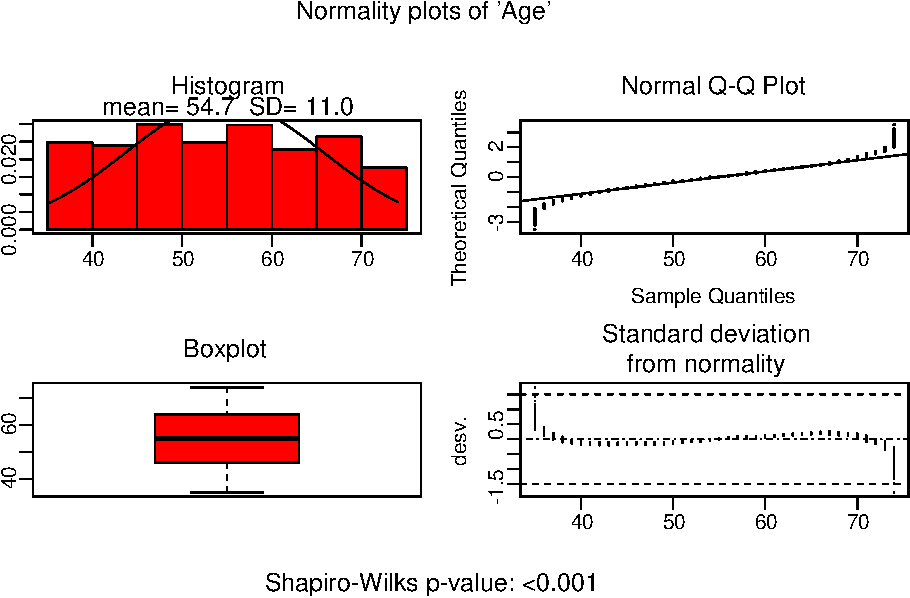
\includegraphics{2-comparegroups_files/figure-latex/unnamed-chunk-16-1.pdf} 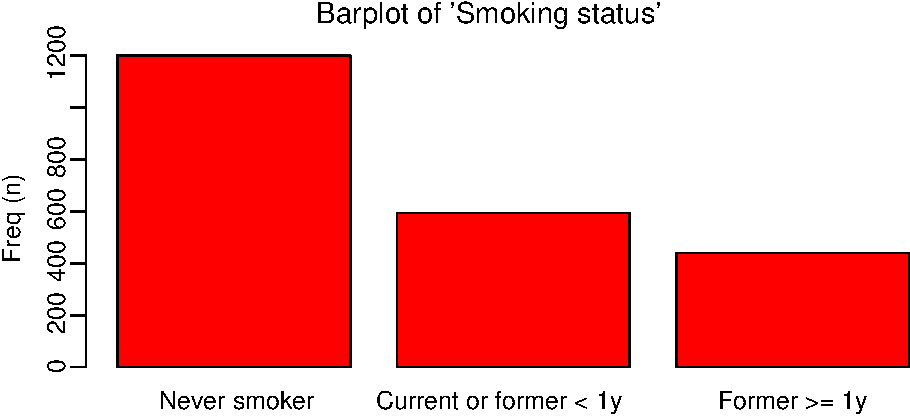
\includegraphics{2-comparegroups_files/figure-latex/unnamed-chunk-16-2.pdf} 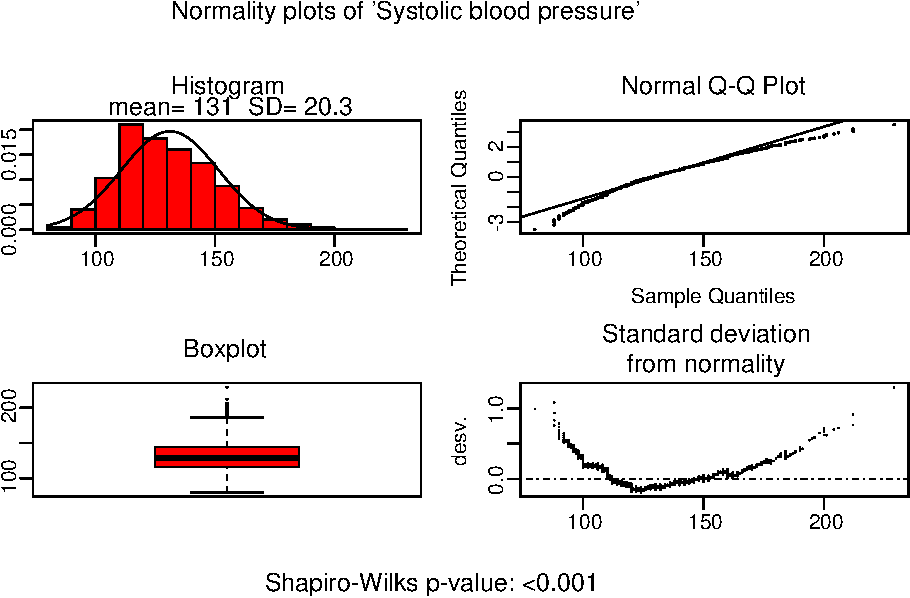
\includegraphics{2-comparegroups_files/figure-latex/unnamed-chunk-16-3.pdf} 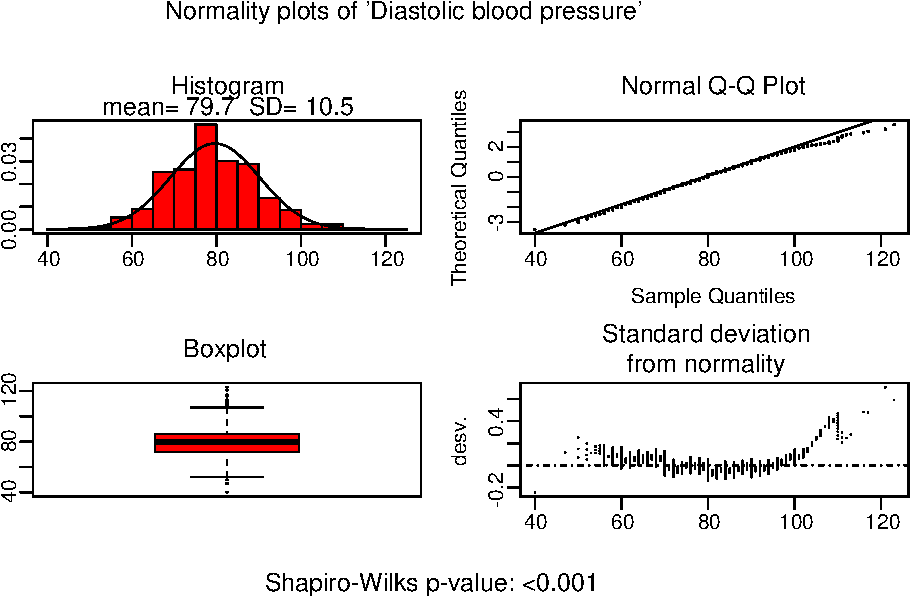
\includegraphics{2-comparegroups_files/figure-latex/unnamed-chunk-16-4.pdf} 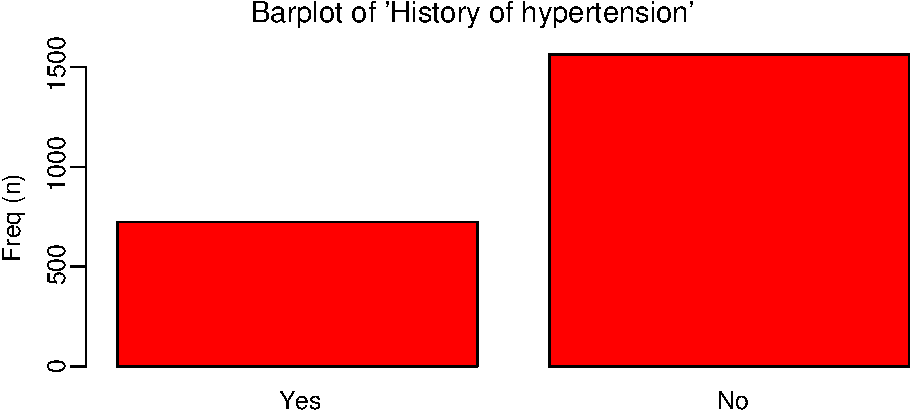
\includegraphics{2-comparegroups_files/figure-latex/unnamed-chunk-16-5.pdf} 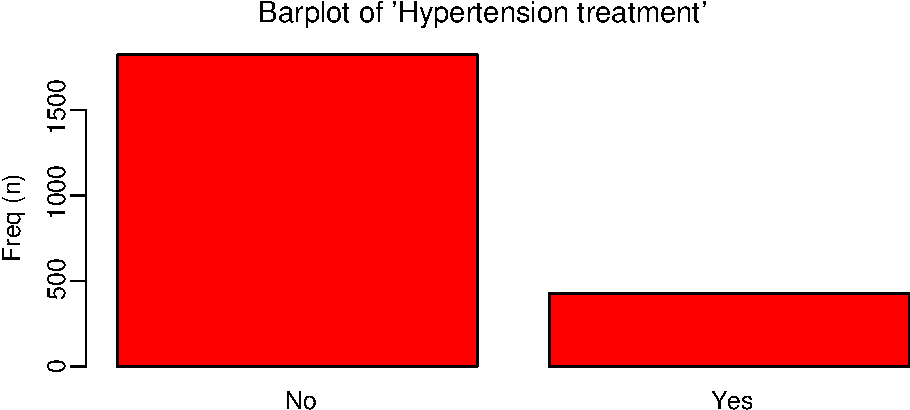
\includegraphics{2-comparegroups_files/figure-latex/unnamed-chunk-16-6.pdf} 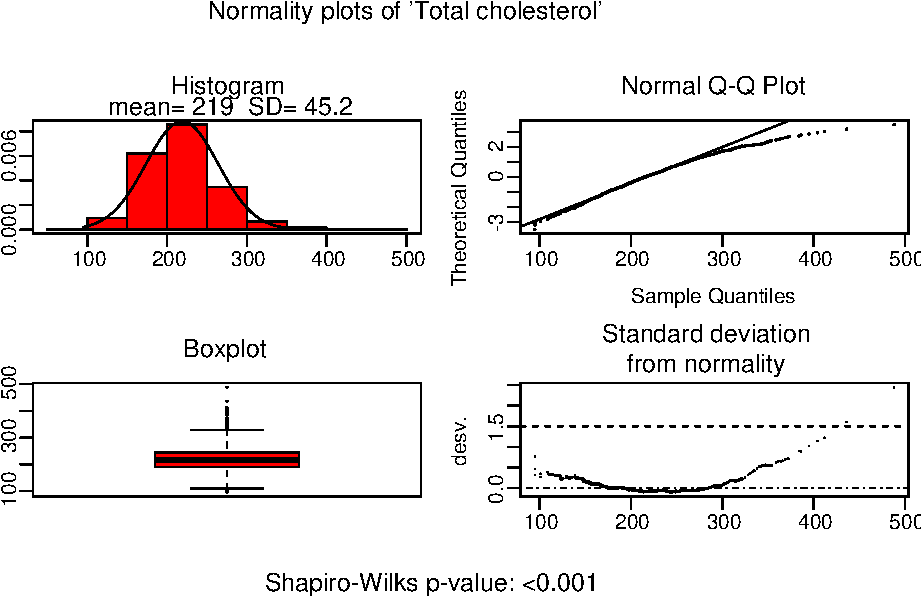
\includegraphics{2-comparegroups_files/figure-latex/unnamed-chunk-16-7.pdf}

\printbibliography

\end{document}
